% Chapter 1

\chapter{Design and Development} % Main chapter title

\label{Chapter3} % For referencing the chapter elsewhere, use \ref{Chapter1} 

\lhead{Chapter 3. \emph{Design and Development}} % This is for the header on each page - perhaps a shortened title

%----------------------------------------------------------------------------------------

%\subsection{Goals}
%\subsection{Observations}
%\subsection{Outcomes, Developments and Improvements}


%Throughout the project nine session were spent The initial sessions centered around introduction of the LeapMotion exploring how it could be used with existing interfaces and designing new interfaces. In the later sessions the application and interface begin to take form and requirements will begin to solidify. 

Throughout the project nine session were spent with KidsTeam. The initial sessions with the KidsTeam centered mostly around the introduction of the LeapMotion. The purpose was to help the children become comfortable with the technology through both brief explanation of how it works and independent exploration. It was important that the children spent time interacting with the technology as early on in the sessions as possible. The more comfortable the children were with using the LeapMotion, the more realistic their creations could be for the interface. 

Later sessions focused on reviewing and improving the application. The application will not be able to make too many drastic design or architectural changes in these later phases.
%Febuary 5th
\section{Session 1: Introduction and Brainstorm}\label{session1}

This first session with the children started with brainstorming ways to use a computer system or control an application without a keyboard and mouse and only using their hands. Using the Bags of Stuff~\ref{sec:bagsofstuff} exercise the children explored designing applications that could only be controlled using gestures.

The children developed several application and game ideas including Pong, Fruit Ninja, Temple Run, Virtual Pet, Internet Explorer, Paint and Maps. The applications were accompanied by many controlling gestures such as a chopstick with button, waving, grabbing, pointing, dragging, pull and release\footnote{Similar to the bird launching interface in Angry Birds}, scratching and striking. 

Afterward the children were allowed to play with a LeapMotion visualizer of the LeapMotion at the end of the session. The visualizer is 3d rendering of what the LeapMotion detects in realtime. 

%\subsection{Goals}

%\subsection{Observations}

%\subsection{Outcomes, Developments and Improvements}

%Feburary 12th 
\section{Session 2: Testing Breakout and Designing a Paint Application}\label{session2}
The children tested a simple BreakOut game which allowed them to interact with the LeapMotion with an application and get a feeling of how it works. With that experience the children were then tasked with designing a painting application that can draw, choose colors and brushes only using gestures to control the interface of their application using the storyboarding~\ref{sec:storyboarding} technique. 

Along with the interface the children came up with several gestures in controlling a variety of user interface controls but most of the gesture controls relied on techniques similar to the way a mouse would function in picking up, dragging and dropping an icons on the screen. Other designs required an action to be performed while pointing at the targeted user interface control indicating a beginning action or ending action\footnote{begin and end actions} instead of waving of a hand, drawing a figure eight in the air or a slashing motion. 

\section{Gesture Design Challenges}
The immediate challenge that faced gestures requiring beginning and ending triggers is how to interpret when each trigger takes place to perform the action. In the mouse and touch screen interfaces the typical design paradigm consists of a beginning action, intermediate action and ending action respectively representing the state in which the input is currently in.

\begin{center}
\captionof{table}{Apple Mac OS X and iOS Application Programming Interface for standard methods of input \cite{appleapi}} \label{tab:title} 
    \begin{tabular}{ | l | l | l |}
    \hline
    Action & OS X & iOS \\ \hline
    Begin  & MouseDown & TouchesBegan \\ \hline
    Moved & MouseDragged & TouchesMoved \\ \hline
    End & MouseUp & TouchesEnded \\ \hline
    Alternate & -- & TouchesCancelled \\ \hline
    \end{tabular}
\end{center}

With the LeapMotion there was no standard way of detecting when each action is to be performed. With this challenge the children came up with the concept of using two fingers to indicate when an action would be performed. Using the thumb as the control mechanism to indicate the action state to be performed and the index finger to indicate the targeted interface control to act upon, the interface control could triggered based on its functionality. The gesture consisted of pulling the thumb flush to the hand while pointing at the user interface control to begin the action and releasing the thumb to indicate the end of the action.With this simple system the a gesture could perform a BeginAction, MovedAction, and EndAction on user interface controls. 


\begin{figure}
\centering     %%% not \center
\subfigure[Open Thumb]{\label{fig:a}
\includegraphics[width=60mm]{HandPointOpen}}
\subfigure[Closed Thumb]{\label{fig:b}
\includegraphics[width=60mm]{HandPointClosed}}
\caption{Hand trigging actions}
\end{figure}

Use case include some of the following control operations

\begin{itemize}
\item Icon Movement pulling the thumb flush to the hand would trigger the BeginAction "pickup" the icon and start dragging it on the screen. The icon could then be placed anywhere on the screen until releasing icon and "dropping" at that position by moving the thumb to a relaxed position no longer flush with the hand performing the EndAction.
\item Selecting a color. The BeginAction would present a popover that would remain open while the user pointed at the desired color until the EndAction. The EndAction would select the color that was pointed at when triggered. 
\item Radio Buttons. A quick BeginAction and EndAction trigger while pointing at the radio button would change the state of the selected item. 
\end{itemize}

\subsection{Implementation Challenges}
In concept this idea seemed to be an ideal and natural way of interacting with the system but faced several challenges. When the thumb became flush with the hand the LeapMotion could no longer detect it as a finger. Additionally, there were several instances of occlusion occurring, for example when the hand was positioned with the thumb pointing upward the line of sight from the camera to the thumb was blocked. This unique challenge was difficult because the thumb could not be accounted for in all cases. An option might be to use the thumb's absence as a trigger although this is prone to many false positives\footnote{False positive indicates a given condition is present when it is not.} when the user's hands were on the boarder line of the LeapMotions visibility range or has lost track of the thumb due to occlusion\footnote{Occlusion occurs when the a surface is hidden by blocking the line of sight.}. Reversing the actions and performing the opposite gesture did not feel natural. Holding the thumb closely to the rest of the hand is not relaxed state and also did not mimic the act of grasping something or triggering an action as people are more commonly used to. 


\subsection{Unity 3D Engine Testing}
Touching two or more fingers together rendered them not recognizable by the LeapMotion and thus would not allow pinch gesture to be used. Alternatives might be calculating when two fingers are close to each other although the LeapMotion cannot differentiate the fingers into which is the index, middle, ring, pinky, and thumb fingers. The application would have to assume any two fingers were performing the gesture and would not allow for the natural separation between fingers unless all fingers were kept folded tight into the hand until needed. 

To observe this behavior a separate project was setup using the Unity 3D Engine to track the different pointers and their interactions in 3D space.\cite{unity}

It was clear after some lengthy prototyping and testing that some of the gestures developed by the children would not be possible and also raised some preliminary speculations that the LeapMotion may only be supplemental in its role except when in application specific situations. Different methods of interacting with these types of controls would need to be developed or would rely on the keyboard and mouse for their functionality.

%%%%%% --- section end

%Feburary 19th
\section{Session 3: Interface Controls}\label{session3}

Common user interface controls were printed out and the children were tasked with brainstorming how they might use LeapMotion to control the widgets or design their own widget that can reproduce the functionality. The user interface controls that we focused on included performing the following tasks were: buttons, drop downs, color palettes, check boxes, radio, buttons, sliders, toggles, steppers, wheels, trees and tabs.

%The user interface controls that have become common and standardized in almost all computer system would need to be adapted or changed to work with the LeapMotion. 

%The user interface controls that required direct text entry would be excluded due to the use of the keyboard although we could not disregard some of the shortcuts that a keyboard provides. In some systems when selecting from a list the keyboard provides a short cut for selecting an item. For example when selecting a the "NJ" for a list of state abbreviations pressing the "N" key will jump to the N section and pressing it repeatedly will cycle in alphabetical order through all of the items starting with letter "N". 
\begin{figure}
\centering     %%% not \center
\subfigure[Carousel view style]{\label{fig:car}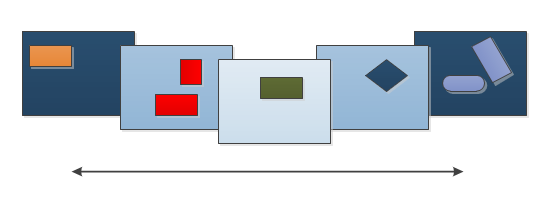
\includegraphics[width=60mm]{car}}
\subfigure[Collection view style]{\label{fig:pan}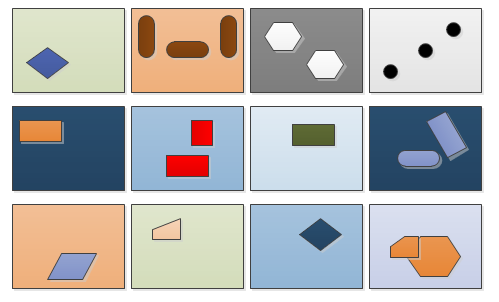
\includegraphics[width=60mm]{pan}}
\caption{Carousel view style maybe zoomed out using a pinch and pull gesture to a collection view. }
\label{fig:collectionview}
\end{figure}
The children did not come up with many new ways of interacting with the user interface controls or developing their own. The main method of interaction focused on pointing to the interface control triggering it using a hand signal with their fingers. The wheel controls could be controlled with flicking motions and dialogs could be dismissed with a wave indicating that the user is finished with the form. Selecting from a list could be done with a list in a carousel view style~\ref{fig:car} where each of the items could be panned through by waving or zoomed out into a collection view style~\ref{fig:pan} of items using pinch and pull gestures. 

Observation of this session reinforced the suspicion that the LeapMotion may not be able to take a role as a dedicated device but as a supplemental device to the mouse an keyboard. Interface controls would also require more space between each of other and to be a of a larger size allowing for a margin of error. Feasible options may include iOS style of modal dialogs which take primary focus until the user in completed with the control. 

%Feburary 26th
\section{Session 4: Testing a drawing application}\label{session4}

Demonstration and hands on testing of a prototype drawing application developed based on the specifications the children had designed in the previous. The children provided feedback using the sticky notes exercise ~\ref{sec:stickynotes} review technique. 

The one requirement that stood out the most early on was the necessity for a Heads Up Display (HUD) which would track where the a pointer is pointing on the screen and also display and interaction with the pointer. Additional features might include motion streaks or gesture animations to provide visual conformation of the action being performed or help the user track where the pointer has been. 

%%Mouse trails paper citation?


%March 5th
\section{Session 5: Designing Gestures }\label{session5}

The children were given some sample gestures and asked to design a way of using the gestures or generate their own for using Microsoft Paint application using the storyboarding~\ref{sec:storyboarding} technique. The sample gestures were turning, tapping, swiping and hand wave. 
\begin{figure}
\centering

\includegraphics[height=1.5in, width=1.5in]{handbox}
%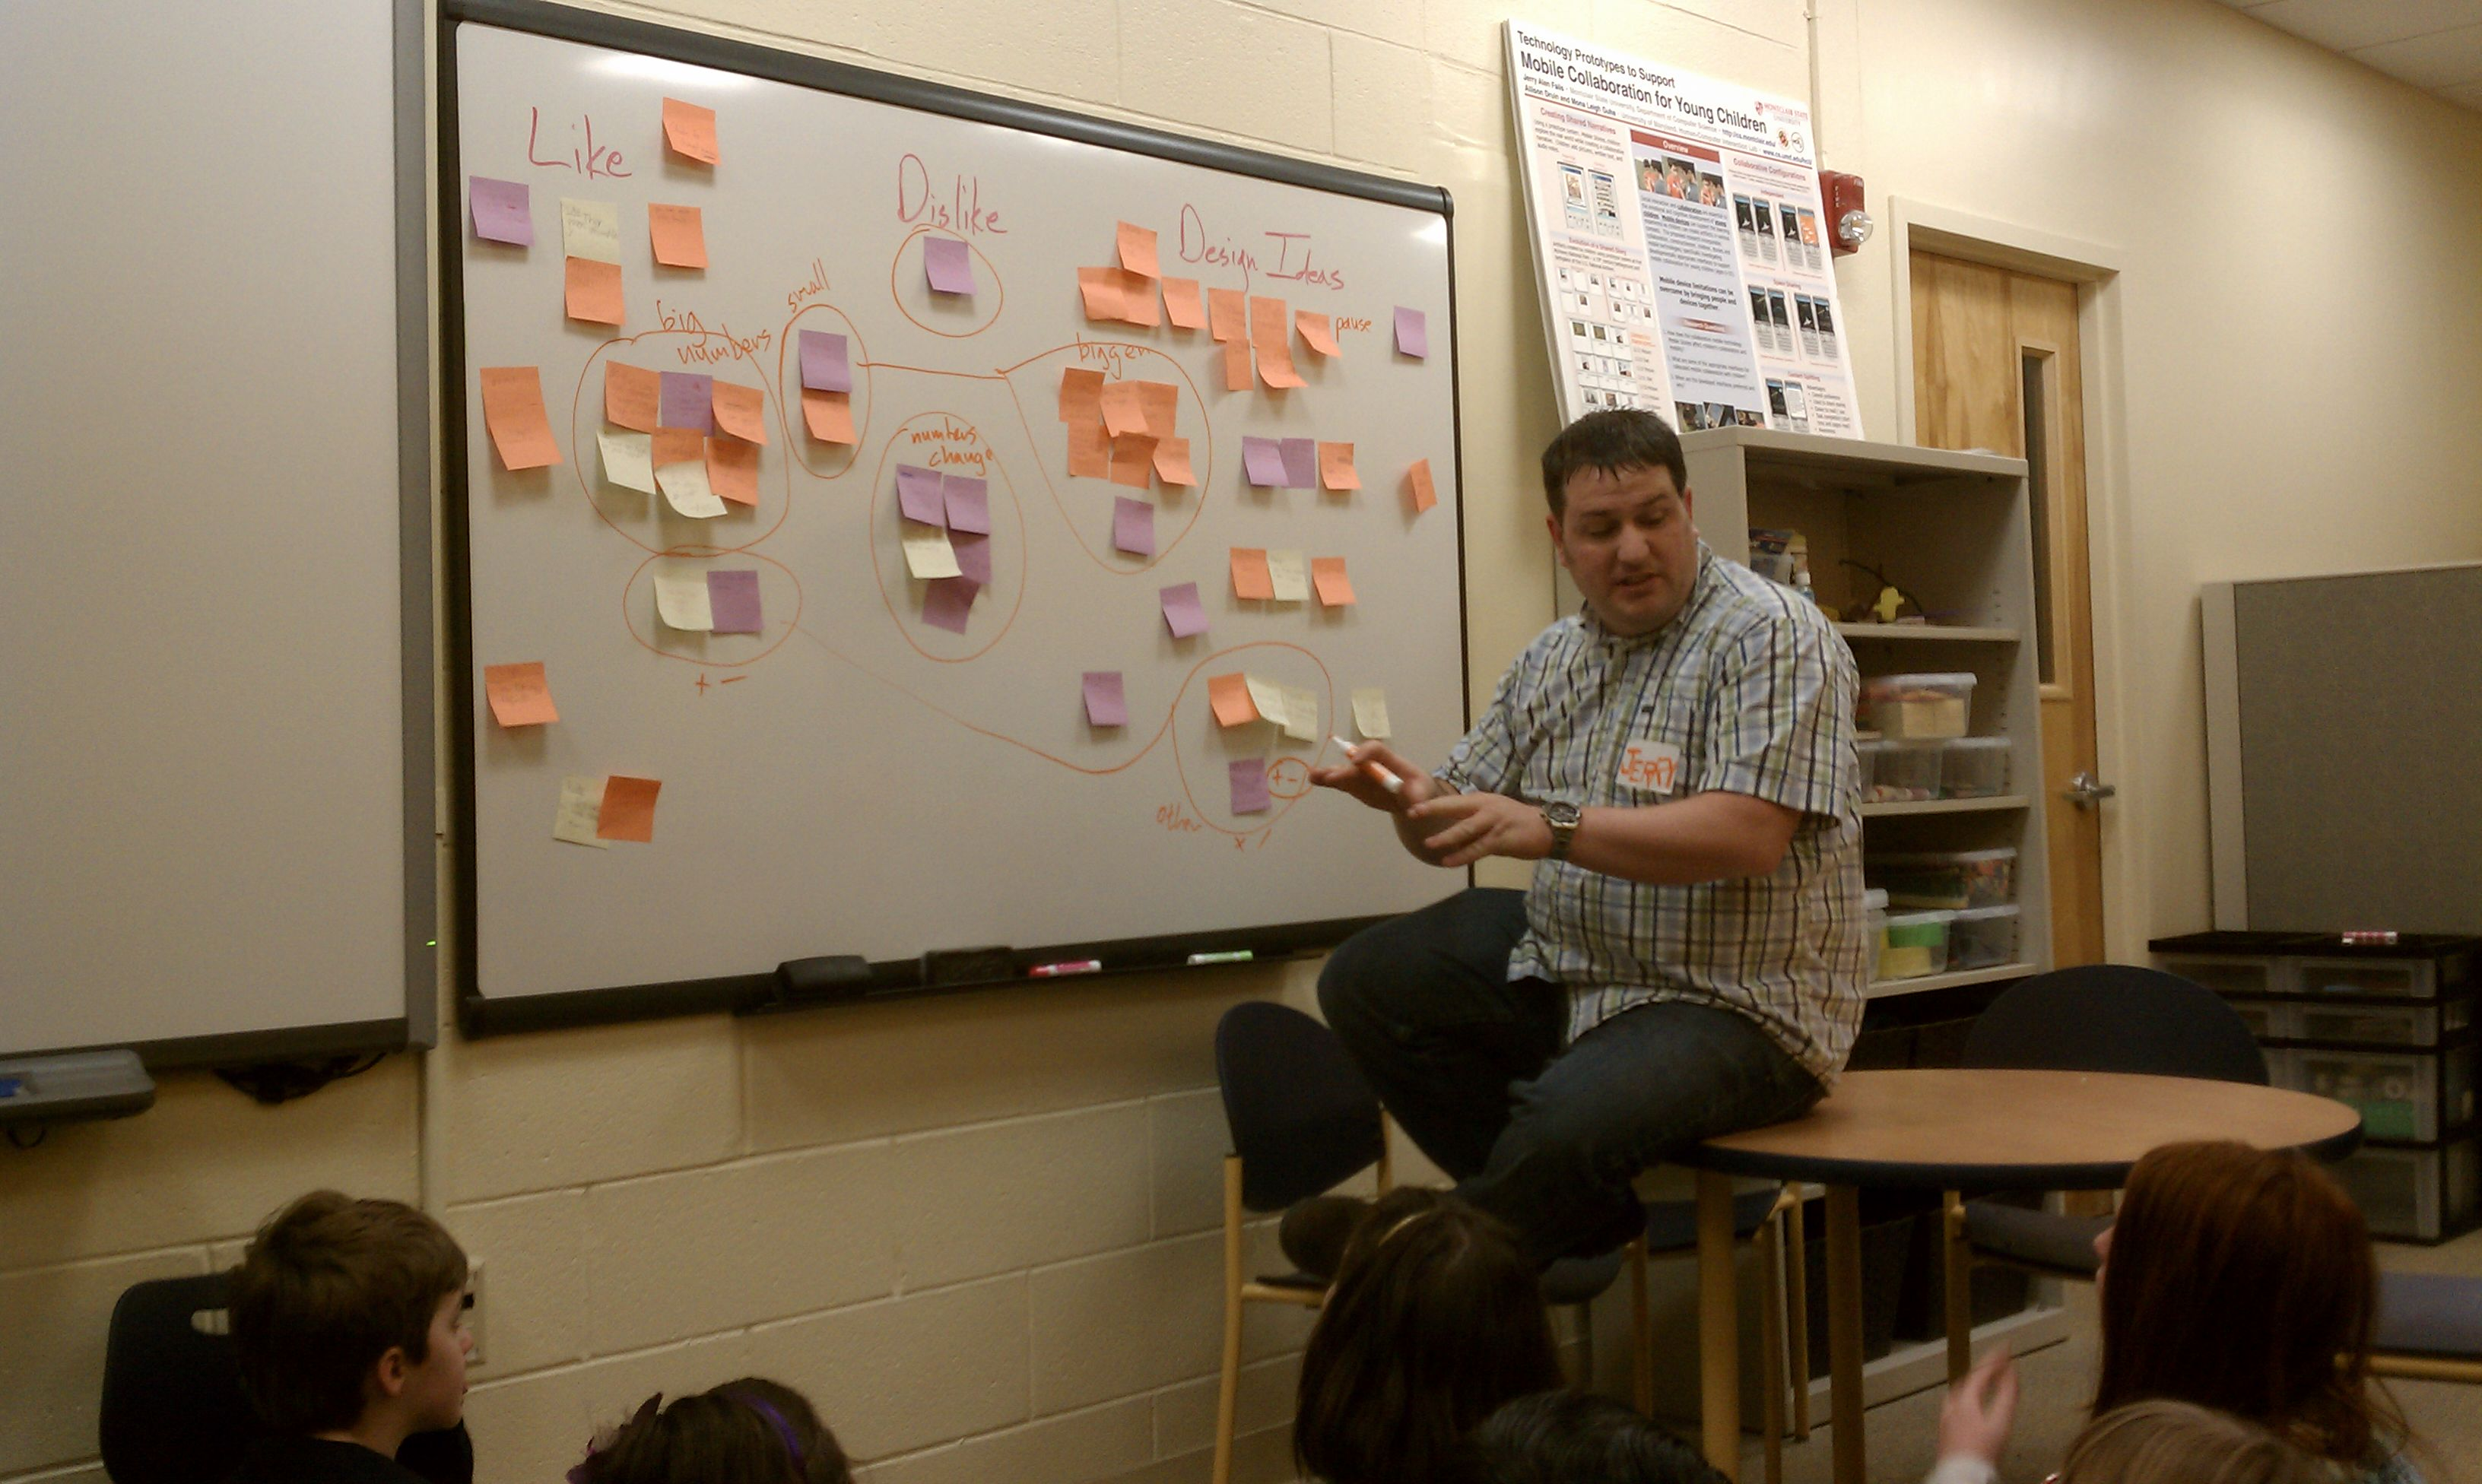
\epsfig{file=IMAG0270, height=1in, width=1.5in}
\caption{Indicating the size of a box by specifying two opposing corners with 'L' shape between the index and thumb fingers.}
\label{fig:handbox}
\end{figure}
Gestures developed by the children were fairly consistent to previous session in pointing to a user interface control and selecting it to perform the action. In the group discussion an idea to use two fingers on two hands to draw the bounds of the box was generated. The finger tips could either represent each of the four corners of the box or two opposing corners by making an 'L' shape as seen in Figure~\ref{fig:handbox}. 

This session reinforced the idea that the LeapMotion cannot be a dedicated device but a supplemental device.

%March 19th 
\section{Session 6: Testing Paint Prototype}\label{session6}


The children were tasked with testing the painting prototype application dubbed LeapPaint using the sticky notes exercise ~\ref{sec:stickynotes} review technique. This early prototype focused on adding a HUD to display the cursor and did not have all of the features in the initial requirements. Testing was focused on the interactions with the cursor. The While not testing they designed their own brushes, shapes and tools to be included in the next iteration of the tool. The overall consensus from this session was to implement better accuracy of the tool which required redesigning how the coordinate systems were translated from LeapMotion space into the application. 

%Go into coordinate systems here performing a vector  triagulation 

%April 2nd
\section{Session 7: Testing Improved Paint}\label{session7}


The children were tasked with testing the painting application with the fixes based on the last session and providing feedback using the sticky notes~\ref{sec:stickynotes} review technique. The new features focused on testing in the application were changing colors, erasing and an experimental method of triggering the drawing action. 

The two different drawing actions were tested with one using the space bar to indicate when to begin drawing. The other used the Z axis of the LeapMotion to begin drawing when breaking a certain plane of depth toward the screen. Children could switch between the modes by pressing the '1' key for space bar mode and the '2' for depth mode and compare each of them.

After testing the children noted that it was difficult to determine where the plane was that would start and stop the drawing actions using the depth mode. The space bar mode seemed to be the preferable option of the two. 

To help the children determine whether they were drawing or not a ring indicator would later be added to show when drawing and not drawing around the cursor by changing from green to red. Additionally the depth mode's flat plane along the Z and X axis would have to calculated as a concave shape for better performance since painting near the edges of the drawing required moving the arm slightly further toward the screen then required in the center. 
%%Figure for this if possible. 


%April 9th Testing and review of the application with sticky notes
\section{Session 8: Final Testing}\label{session8}

The children were tasked with testing the painting application for the last time using the sticky notes~\ref{sec:stickynotes} review technique. Testing for new features which included a depth opacity control. The opacity of the brush would become greater the closer the pointer was to the monitor simulating how a paintbrush or marker makes a darker line when pressed harder to paper. 

The children preferred the method of using depth to control the opacity over performing the manual adjustments with the mouse. 
\begin{figure}
\centering     %%% not \center
\subfigure[]{\label{fig:car}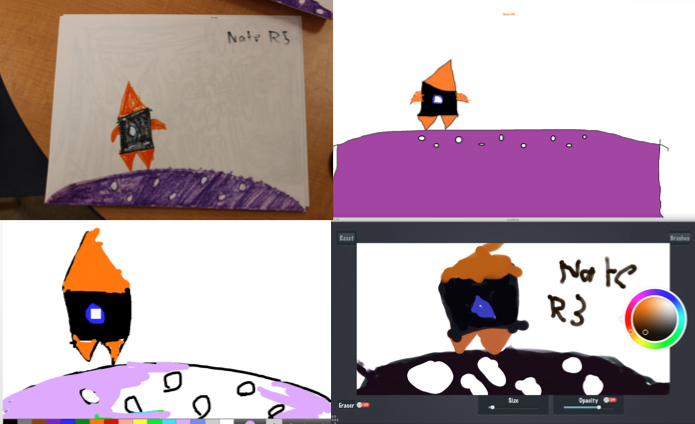
\includegraphics[width=60mm]{compare1}}
\subfigure[]{\label{fig:pan}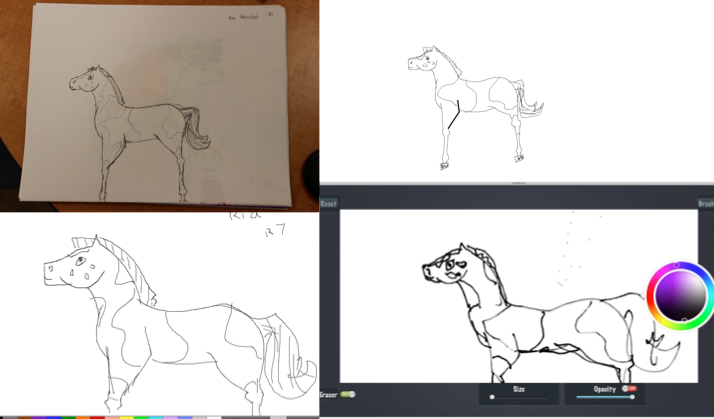
\includegraphics[width=60mm]{compare2}}
\caption{Drawings done by hand (top left), in Microsoft Paint (top right), on the iPad (bottom left) and with the LeapMotion (bottom right)}
\label{fig:comparisondrawing}
\end{figure}

%April 15th
\section{Session 9: Usability Comparison}\label{session9}
The last session compared the LeapPaint application with a three different methods of drawing with different interfaces. The children were given the task of drawing the same picture of their choice on each system. Each child was given 10 minutes of time to attempt to reproduce a drawing by hand drawing using markers, Microsoft Paint using a mouse and keyboard, SimpleDraw on the iPad's touch interface and with LeapPaint using the LeapMotion. 

The resulting drawings were mixed in comparison but showed that the drawing ability in the application may be related to the amount of time the child has had using the application. Drawing comparisons can be seen in Figure~\ref{fig:comparisondrawing} by two different children. 



